\documentclass[12pt, letterpaper]{article}
\usepackage[letterpaper, portrait, margin=1in]{geometry}
\usepackage[utf8]{inputenc}
\usepackage[english]{babel}
\usepackage{graphicx}


\begin{document}

\title{%
\huge \textbf{Project Barker}\\
\large An Art Project on Social Media, Intelligent Machines, and Reality}

\author{Leo Lin, Minh Nguyen}

\maketitle

\newpage
\abstractname{ -- Project Barker is an art project that comments on the current reality of social media and human-computer interactions. Generation technology involving multiple state-of-the-art (SOTA) models helps us to build a completely "fake" Twitter. Through this interactive medium, we hope to not only trigger contemplation regarding the often underestimated power of social media and the meaning of the difference between modern social media and conventional communication technologies but also provide a space to examine humanity in front of intelligent machines and explore the boundary between the virtual world and the reality.}

\section{Introduction}

\paragraph{Social Media}Social media has become a serious societal force. It has enabled some positive change and played important roles in mass movements, such as the recent BLM movement. It also accelerates the spread of disinformation and conflict. Its potential is, so far, underestimated by the general public. Malicious entities have exploited these platforms to promote conspiracy theories, influence elections, and exacerbate genocides.

\paragraph{Artificial Intelligence}Artificial Intelligence has also profoundly impacted the world. It has transformed the medical industry, for example, with better-than-human diagnoses using computer vision and protein folding to assist drug design. However, combined with social media (in reference to recommendation algorithms), it has created echo chambers and promoted sensationalism and fake news.

\paragraph{Project Barker}Seeing that, we wanted to create a genuine yet almost satirical representation of social media and AI. Barker is a half-fledged antisocial media platform filled with AI-generated content that mimics the design of Twitter. It is not a piece of art to be marveled at, but one to experience. Exploring the app reveals information about the content’s sources and inspirations, and reading the content itself reveals not only the nature of the internet but the viewer’s very mind.

\section{Process}

\subsection{Leo Lin}

\paragraph{}My work mainly focuses on working with the various AI Models to produce the various types of images that were needed for the project. I've gathered and processed data and studied new models. I've also experimented with building my own video-generation models.

\paragraph{Image Generation}The part of my work that contributed to the final product the most is image generation. I've trained StyleGAN on multiple datasets I collected myself: emoji, Trump, Time covers, and Chinese characters. I've utilized pre-trained models such as BigGAN and AttnGAN to produce images for the final product. 

\paragraph{Data Processing}Like mentioned above, I had to collect most of the data for training the desired models. The new skills I learned includes basic web crawling and font file processing. Through the process of writing code for processing JSON files, transform images, filter texts, etc. I greatly improved my coding skill (in terms of data/file processing) with these experience.

\paragraph{Learning}Despite having experience with Deep Learning, I was relatively new to the realm of Natural Language Processing (NLP). So I spent many hours on teaching myself the concepts and structures SOTA NLP models (mostly Transformers). I read many papers including Transformers, BERT, ELmo, Big Bird (yes these models are actually called that, I didn't spend my SSTP watching Sesame Street), Longformer, Reformer, StyleGAN, CycleGAN, and many others to teach myself the new progresses in the field.

\paragraph{Experiments}I've also spent a lot of time attempting to construct a video-generation model based on the reformer structure with a new token mechanism. I had to abandon this plan due to the lack of time but it was a very exciting opportunity to experiment with the things I've just learned. I did not really expect this to work (my paper would be in ICCV if it actually did, video-generation is a very cutting-edge topic that still lacks satisfactory results) but the knowledge and experience I gained was totally worth the time spent.

\paragraph{Misc.}I've also gained some new experience with other rather minor things. I gained more experience with cloud computing (more time on MatPool and Google Colab, explored Kaggle, Runway ML) as most of my previous work were run on my personal node. In working with Minh, we tried to setup a remote forwarding server and an FTP server for better efficiency (an effort which Mr. Mandel also joined). I've learned how to use GitHub to manage code between multiple collaborators (all my previous use are for my own backup). I've also explored the field of video game design during the early stages of the project where we were trying to produce a film. This pursuit also sparked a conversation with Tim Oxton, a part-time photographer and video game developer.


\subsection{Minh Nguyen}

\paragraph{}My work revolves around making Barker app and its text content. I learned to be a super-full-stack developer from knowing nothing about web developement. Previously, I learned programming languages and frameworks the "proper way," as in, I took an intro class (or an entire course in the case of Java in AP CS-A). Because of the short time that the SSTP allows, I had to come in blind. It was an interesting experience, to say the least. Additionally, I've become better at manipulating deep learning models. 

\paragraph{Barker Frontend}The app's frontend is made using the React framework in JavaScript (JS). Before this project, I did not know JS, let alone used a web development framework. Furthermore, I have never had any experience in the visual arts---or HTML and CSS, which is the programming for the app's appearance---which made developing a user interface (UI) a challenge. I experienced different ways to think about programming. A lot of JS happens asynchronously which makes it feel very non-procedural. Thinking about a program in terms of sub-programs that can overlap and oftentimes interfere with each other is unlike anything I have done yet is necessary with any people facing program. Using a developement framework, React, I gained valuable experience in what it is like to be a software developer. I learned to adapt to the "quirks" and "imperfections" in the system itself. Trying to execute my plans for the site's appearance using HTML and CSS was the most frustrating that was nevertheless informative. They work through sugggestions-based descriptions of what I want, instead of hard commands that I can compel, which was an analogue of how real life works. Making the front end spoke the most to the "interesting experience" to which I referred. I also have a lot more appreciation for the designers of UI/UX, about which I often complain.

\paragraph{Barker Backend}The app's backend is made using the Django framework in Python and hosted on Google Cloud Platform's (GCP) App Engine (AE). The data is stored in an embedded Structured Query Language (SQL) database. I did not know Django beforehand (since I never used a web development framework), but I did know Python. It was helpful that I knew the language, but it did not help as much as I anticipated. I came in complacent and did not defer as much to tutorials, which was unwise. I had to wrestle with Django, SQL, and \emph{the Internet} and the lack of help for it online, despite it being almost as old as me. Internet protocols were restricting and made things more complicated; I had to be careful as to not allow the user to be attacked (though I, as the developer, am not at risk thanks to hosting on AE). I especially struggled with designing and manipulating the database because I did not even know the design and functional patterns of SQL---it was like driving a car without knowing what roads are. Fortunately, Django and SQL's age means that they are much more stable and reliable, though I did almost completely mangled my database were it not for version control. The difficulty in programming is not the programming language but the thought and design that goes behind it. Not that I didn't know it (after all, I'm not substituting my college degree with a programming course), this was definitely the most powerful example I've experienced.

\paragraph{Text Generation}I trained OpenAI's GPT-2, a Natural Language Processing model, on various text content sources. I trained the model to replicate Tweets from the Russian campaign to influence the 2016 election, Tweets representative of Twitter as a whole, and news articles from major online publishers. The scraping (collection of data from the sources themselves) was done by people more qualified than me. Nevertheless, I have become more experienced in data transferring and processing through extracting and refining data from the datasets.

\paragraph{Lessons}To the ends of making the product, we failed many times. For example, we spent a considerable amount of money and effort to modify and train AI models that we never used in the end. However, I do not consider it to be a waste of either. Cloud computing is a resource that I will almost definitely use in the future in my planned career. If I choose the path of AI, the experience of programming with and around AI models, albeit frustrating, will be quite useful. Most importantly, I am mure assured that I have made the right choice in my chosen career field. Even though I may regret the opportunity cost, I do not lament having spent many a nights wrestling with React, Django, GPT-2, StyleGAN, or MatPool. 

% Are we gonna bother with this?
\section{Product Structure} 

\section{Conclusion}

\paragraph{}In making the app and “creating” the content, we have improved our skills in data science, programming, and UX design. More importantly, however, we learned so much about ourselves. In reading the generated content, we explored our own thoughts and easily manipulated they are. In working on the project, we gained valuable experience with working in a team in a technical project as well as insight into what we do and do not want to do in our future careers.

\section*{Appendix}

\begin{figure}[h]
	\begin{center}
		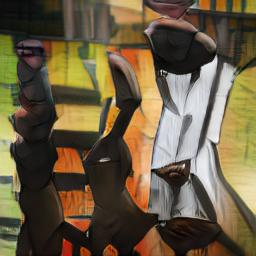
\includegraphics[width=\linewidth]{imgs/000001075.jpeg}
    		\caption[width=\linewidth]{image we have generated using Attention GAN}
    		\label{AttnGAN}
	\end{center}
\end{figure} 

\end{document}
